\chapter{Implementation}\label{implementation}
\section{Data Collection and Exploration}
In order to train the neuro-fuzzy controller, data from the simulation using PID controller was collected. To reduce overfitting and to train the controller for all scenarios, the simulations from which data was to be collected had randomised waypoints and obstacles. The data from 40 simulations each with a sample rate of \SI{0.01}{\second} was collected giving a total of 505,075 datapoints, representing \SI{84}{\minute} of drone operation.  
 
There were 18 inputs and 4 outputs collected, shown in Table \ref{tab:inputsOutputs}.
\begin{table}[H]
    \centering
    \begin{tabular}{@{}llll@{}}
        \toprule
        \textbf{Inputs}& & \textbf{Outputs}&\\
        \midrule
        Time & (\si{\second})                   & Roll Control Signal &(\si{\radian\per\second})  \\
        Desired $x$ Position & (\si{\meter})           & Pitch Control Signal &(\si{\radian\per\second}) \\
        Desired $y$ Position & (\si{\meter})           & Yaw Control Signal &(\si{\radian\per\second})   \\
        Desired $z$ Position & (\si{\meter})           & Thrust Control Signal &(\si{\meter\per\second})  \\
        Desired Yaw & (\si{\radian})                &       &                       \\
        Actual $x$ Position & (\si{\meter})            &    &                          \\
        Actual $y$ Position & (\si{\meter})            &   &                           \\
        Actual $z$ Position & (\si{\meter})            &   &                           \\
        Velocity $x$ & (\si{\meter\per\second})                 &    &                          \\
        Velocity $y$ & (\si{\meter\per\second})                 &    &                          \\
        Velocity $z$ & (\si{\meter\per\second})                 &   &                           \\
        Roll- Body Angular Rate & (\si{\radian\per\second})  &    &                          \\
        Pitch- Body Angular Rate & (\si{\radian\per\second}) &     &                         \\
        Yaw- Body Angular Rate & (\si{\radian\per\second})   &     &                         \\
        Roll- Euler Angle & (\si{\radian})          &     &                         \\
        Pitch- Euler Angle & (\si{\radian})         &     &                         \\
        Yaw- Euler Angle & (\si{\radian})           &     &                         \\
        Thrust & (\si{\meter\per\second})                 &    &                             \\
        \bottomrule
    \end{tabular}
    \caption{List of inputs and outputs.}
    \label{tab:inputsOutputs}
\end{table}
In order to understand the dataset, various time series graphs were plotted. As the dataset was extensive, the relationships were difficult to identify. Therefore, sections of data were analysed and plotted instead of using the whole dataset so as to understand the relationship between certain variables. These are shown in Figures \ref{fig:thrust_plot}, \ref{fig:yaw_plot}, \ref{fig:pitch_plot}, \ref{fig:roll_plot}, \ref{fig:x_plot}.
\begin{figure}[H]
    \centering
    \begin{minipage}[b]{0.45\textwidth}
        \centering
        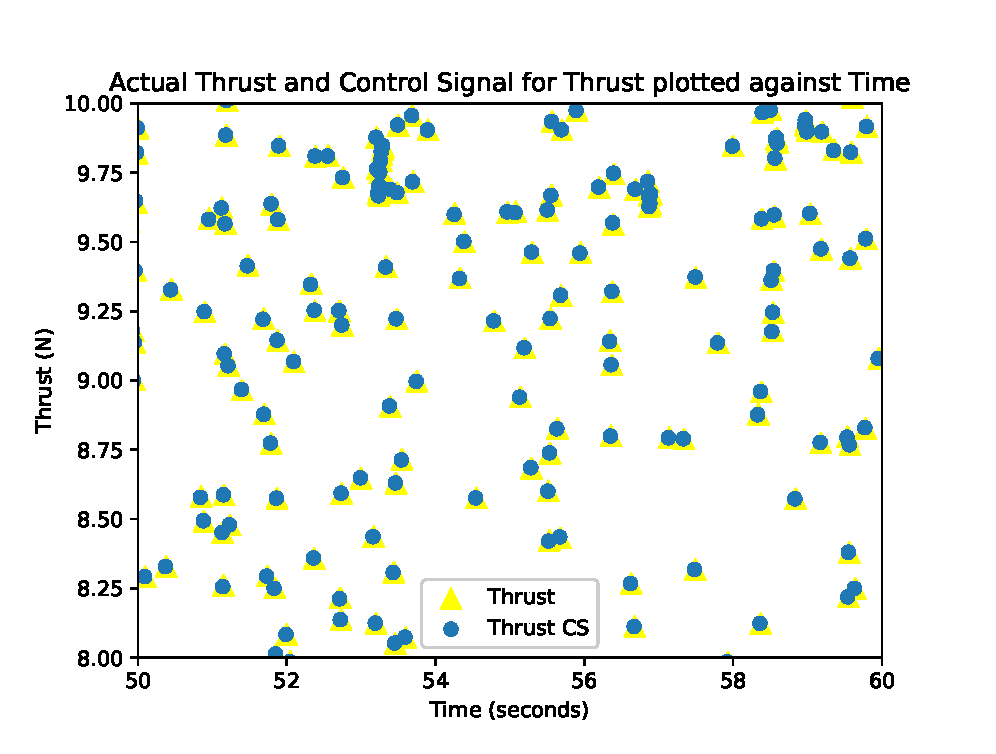
\includegraphics[height=5.5cm,keepaspectratio]{img/thrust_plot.eps}
        \caption{Actual thrust and control signal for thrust plotted against time}
        \label{fig:thrust_plot}
    \end{minipage}
    \hfill
    \begin{minipage}[b]{0.45\textwidth}
        \centering
        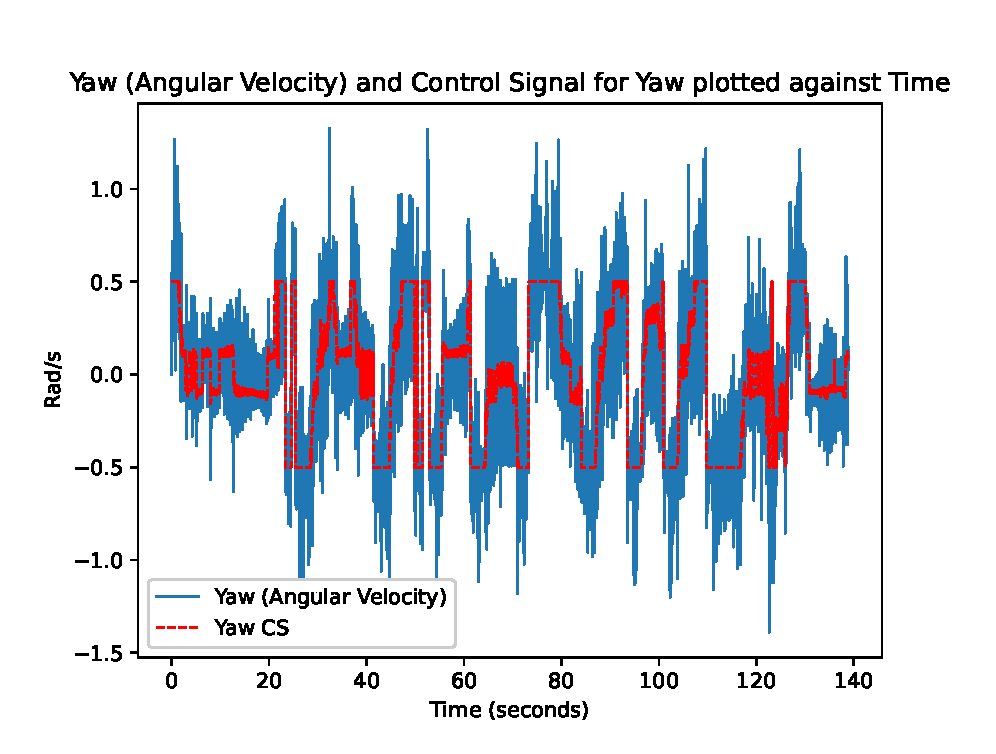
\includegraphics[height=5.5cm,keepaspectratio]{img/yaw_plot.eps}
        \caption{Yaw (angular velocity) and Control Signal for Yaw plotted against time}
        \label{fig:yaw_plot}
    \end{minipage}
\end{figure}
\begin{figure}[H]
    \centering
    \begin{minipage}[b]{0.45\textwidth}
        \centering
        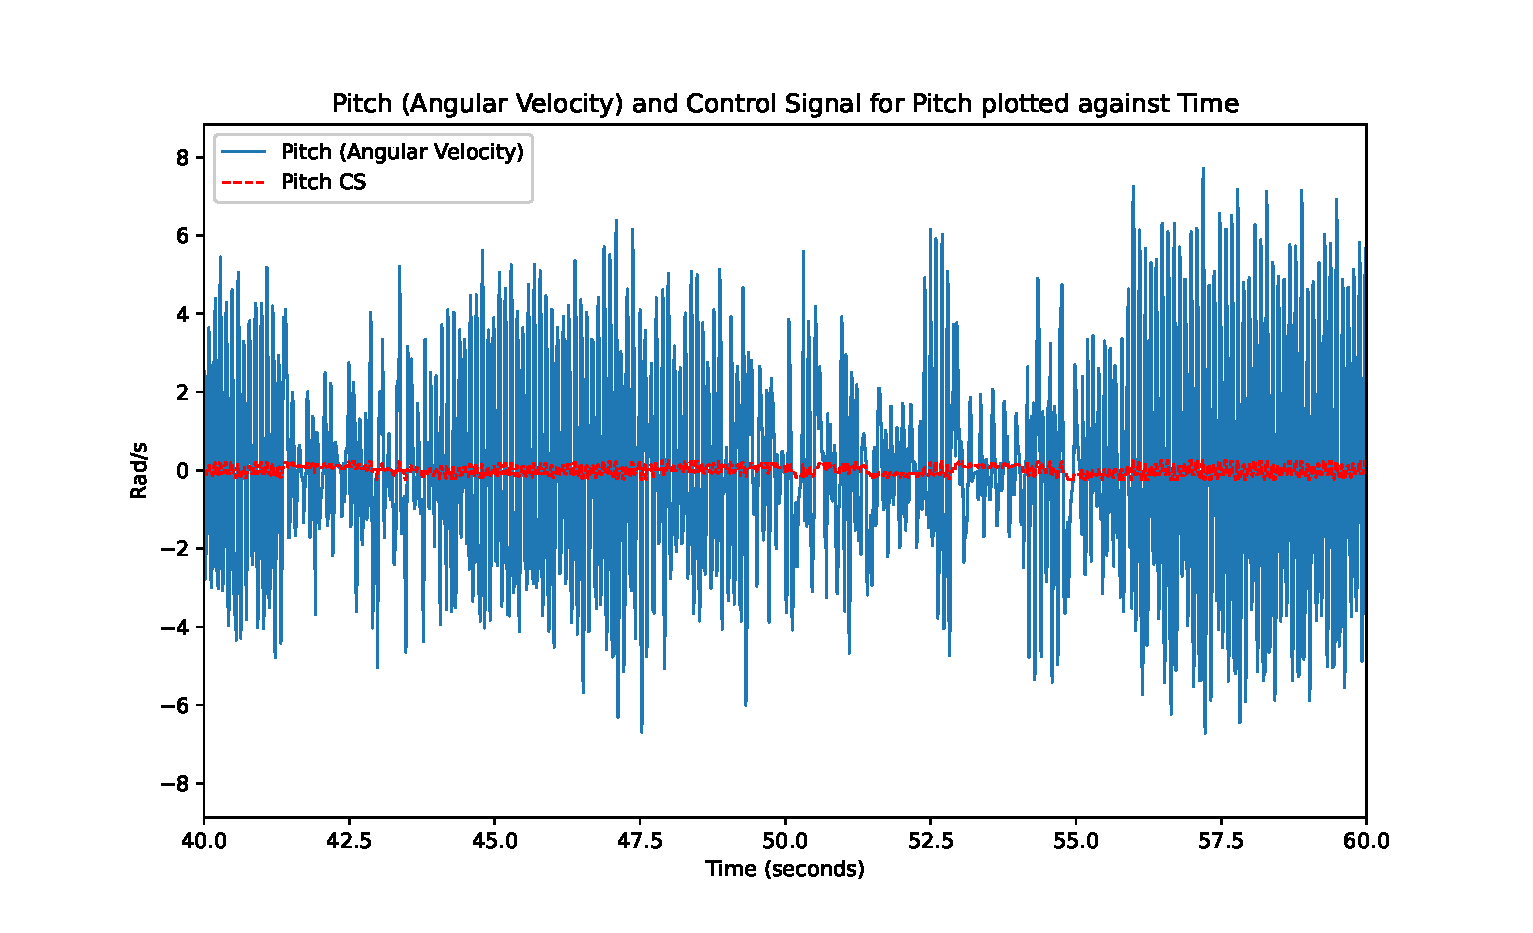
\includegraphics[height=5.5cm,keepaspectratio]{img/pitch_plot.eps}
        \caption{Pitch (angular velocity) and Control Signal for Pitch plotted against time}
        \label{fig:pitch_plot}
    \end{minipage}
    \hfill
    \begin{minipage}[b]{0.45\textwidth}
        \centering
        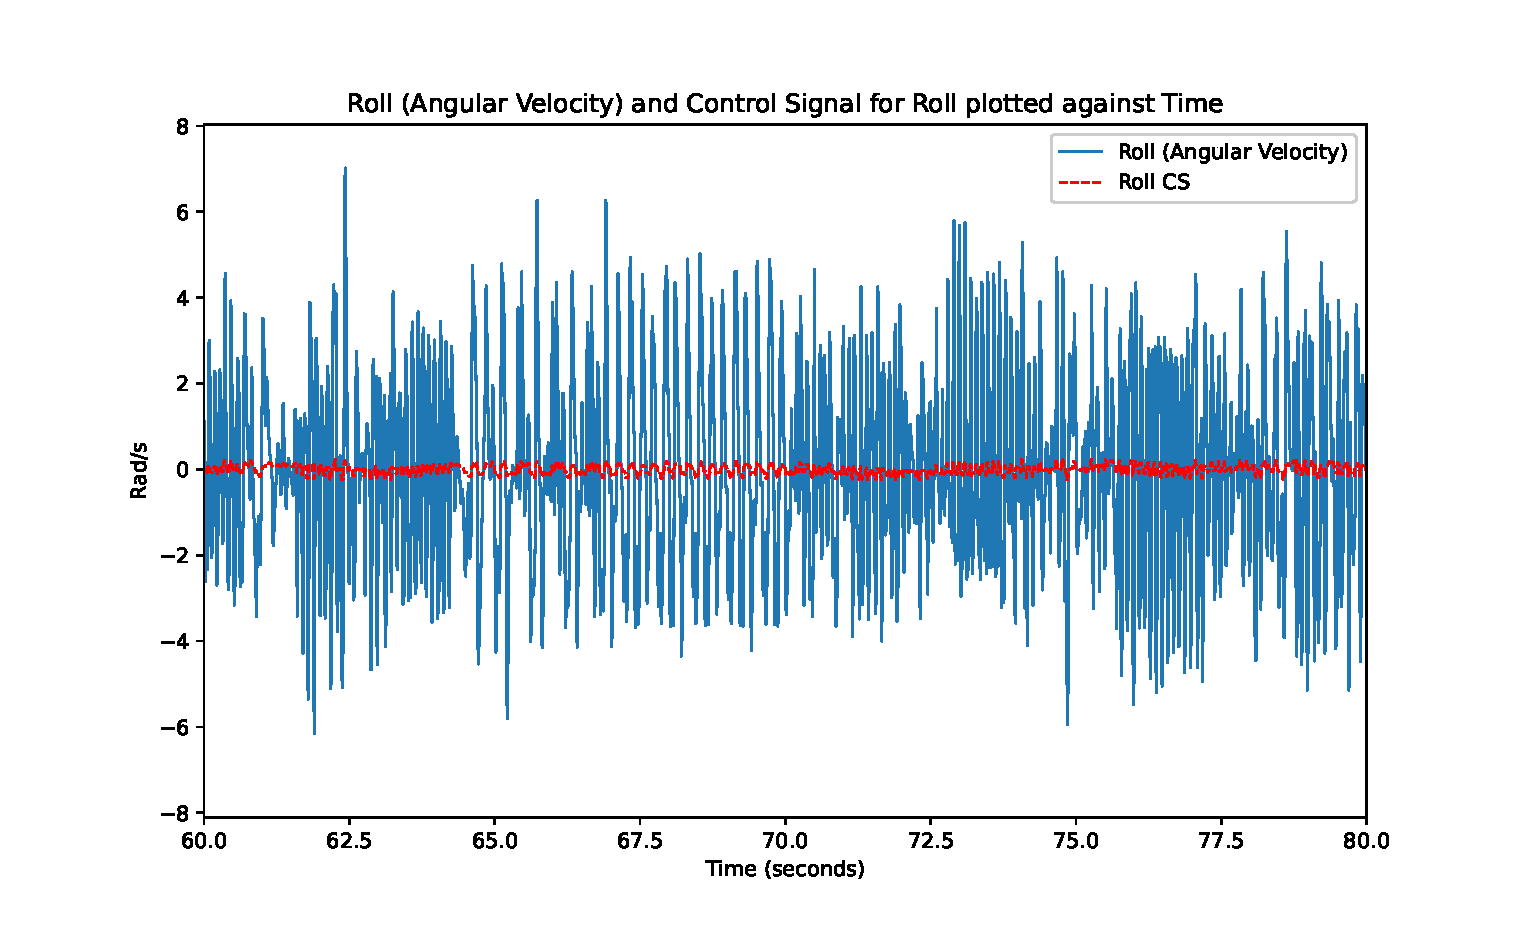
\includegraphics[height=5.5cm,keepaspectratio]{img/roll_plot.eps}
        \caption{Roll and Control Signal for Roll plotted against time}
        \label{fig:roll_plot}
    \end{minipage}
\end{figure}
\begin{figure}[H]
    \centering
    \begin{minipage}[b]{0.45\textwidth}
        % empty minipage
    \end{minipage}
    \hfill
    \begin{minipage}[b]{0.45\textwidth}
        \centering
        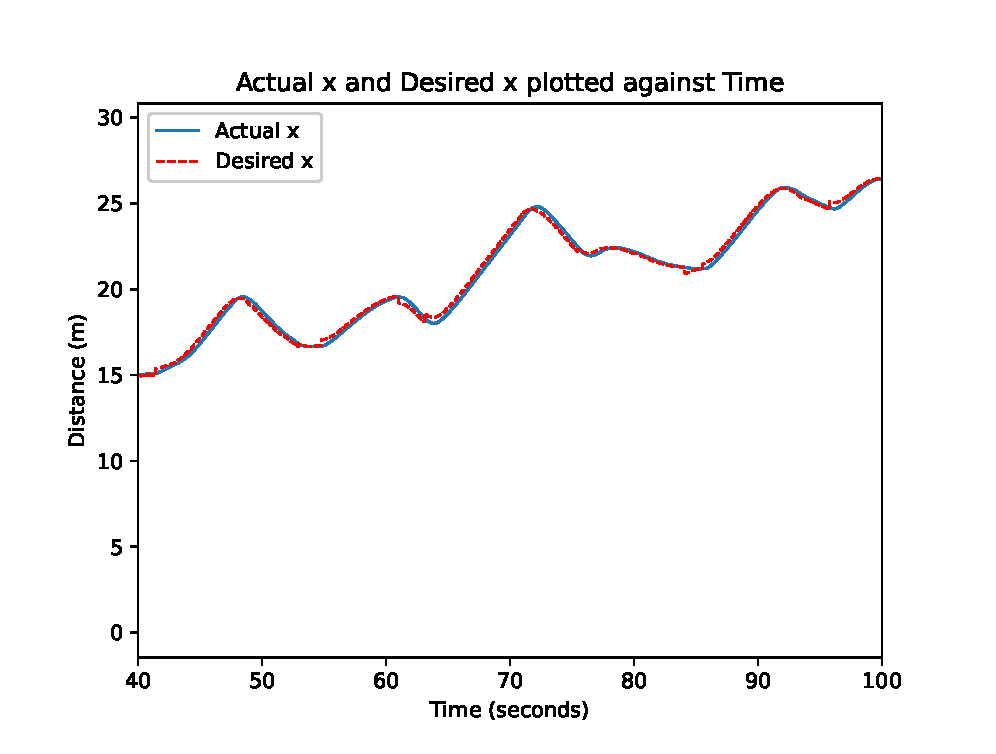
\includegraphics[height=5.5cm,keepaspectratio]{img/x_plot.eps}
        \caption{Actual position x and desired position x plotted against time.}
        \label{fig:x_plot}
    \end{minipage}
    \hfill
    \begin{minipage}[b]{0.45\textwidth}
        % empty minipage
    \end{minipage}
\end{figure}
Figure \ref{fig:thrust_plot}  shows that the actual thrust value and the control signal are almost equivalent in most cases. Figure \ref{fig:yaw_plot} shows the yaw control signal is often discrete at either \SI{0.5}{\radian\per\second} or \SI{-0.5}{\radian\per\second}, which makes intuitive sense due to yaw representing a significant alteration in the drone’s direction of travel. Figures \ref{fig:pitch_plot}  and \ref{fig:roll_plot} are similar and show that the pitch and roll values are subject to more continuous variation. As seen from Figure \ref{fig:x_plot} the actual $x$ value for the drone closely follows the desired $x$ value as expected. The difference between these values is a key indication of the performance of the drone and will be discussed in Chapter \ref{chapter5}. 
\section{Feature Selection and Engineering} \label{feature selection}
Feature selection and engineering is an important step when training any machine learning system. 

Despite time, $t$, being part of the set of inputs shown in Table \ref{tab:inputsOutputs}, it is not used by the drone and is not relevant to the training of the drone, the time variable was removed. This reduced the number of inputs down to 17. Due to the Simulink drone model using all the remaining 17 inputs in its controller, any feature selection and engineering would mean the model must be altered accordingly, such that the controller is fed the same inputs as the neuro-fuzzy controller is trained on. Therefore, only limited feature engineering and selection was carried out.  

Absolute measures that were not relative to the drone's movement are not useful to the learning based system. As a result, desired position and actual position both are absolute measures therefore this information was not helpful for the neuro-fuzzy controller. Instead, the difference between the desired position and actual position is of relevance. Therefore, the following feature engineering was performed: 
\begin{align}
    x_{\textrm{desired}} - x_{\textrm{actual}} & = x_{\textrm{desired change}}\\
    y_{\textrm{desired}} - y_{\textrm{actual}} & = y_{\textrm{desired change}}\\
    z_{\textrm{desired}} - z_{\textrm{actual}} & = z_{\textrm{desired change}}
\end{align}
This resulted in the number of inputs further decreasing from 17 to the 14. Reducing the number of inputs further would require appropriate adjustments to the Simulink model which could lead to computational inefficiencies. Despite this, it was important to check if there were any unnecessary features in order to not waste computational power. The filter feature selection method was applied to check this. This method is very useful for machine learning models with numerical inputs and outputs. The filter feature selection method chosen was the Pearson Correlation Coefficient method where the Pearson coefficients were analysed and a heatmap of the correlation between the features was created. This can be seen in Figure \ref{fig:zain6}. The features with highest correlation were the velocities in the $x$, $y$ and $z$ direction and their corresponding desired changes in the $x$, $y$ and $z$ directions. As found in literature, a correlation coefficient greater than 0.85 demonstrates a strong correlation and consequently should be removed \cite{654654}. Since we did not have any features with correlation coefficients greater than 0.85, no features were removed and all were deemed to provide relevant information to the fuzzy inference system.
\begin{figure}[H]
    \centering
    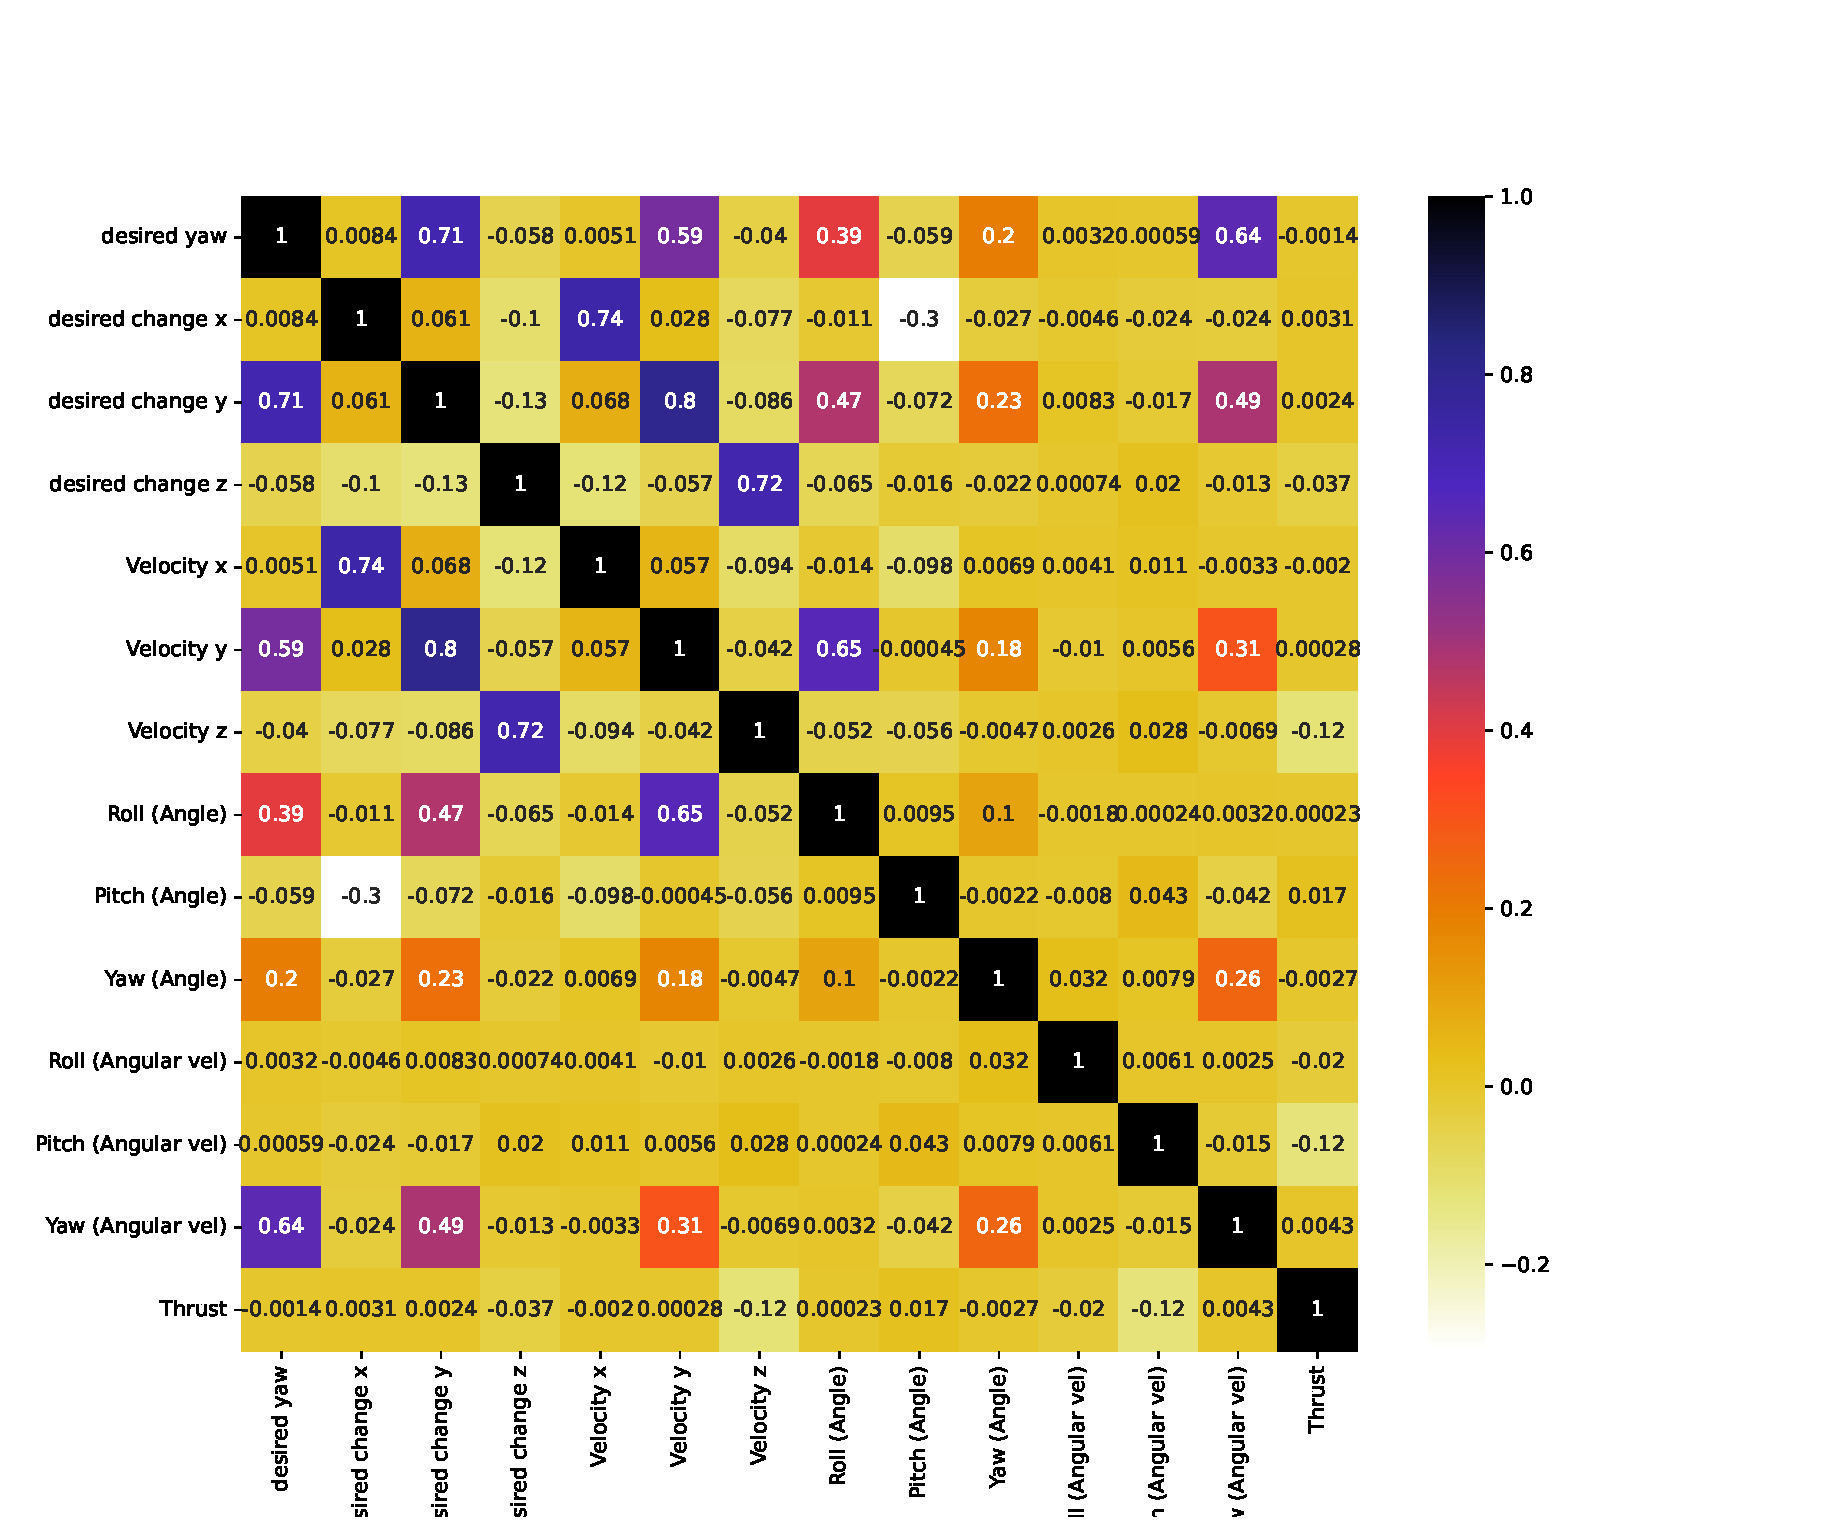
\includegraphics[width = 0.7\textwidth]{img/pearson.eps}
    \caption{Pearson correlation coefficient heatmap.}
    \label{fig:zain6}
\end{figure} 
\section{ANFIS Configuration}
There may be instances of natural phenomena that inherently possess a degree of indeterminacy, making them difficult to accurately model without embracing some level of non-probabilistic uncertainty. One technique to address this ambiguity is the application of fuzzy logic. Fuzzy values or fuzzy sets do not adhere to strictly defined numerical limits, often referred to as sharp boundaries. Rather, these boundaries tend to gradually fade in the context of fuzzy sets. In general, a Sugeno-type inference system is proposed, with the resultant parameters of the fuzzy rules presented as a polynomial function: 
\begin{align}
    &\texttt{if } X \subset A \And Y \subset B\\
    &\texttt{then } Z = f\left(X,Y\right)\\
    &\texttt{where } f\left(X,Y\right) = pX + qY + r
\end{align}
For the purpose of simplicity, consider a fuzzy inference system with two inputs labelled $X$ and $Y$, as well as a single output labelled $Z$. It is assumed that the rule base consists of two fuzzy if-then rules organised in accordance with Takagi and Sugeno's type \cite{TAKAGI198355}.

Rule 1:
\begin{align}
    &\texttt{if } X = A_1 \And Y = B_1\\
    &\texttt{then } f_1 = p_1X + q_1 Y + r_1
\end{align}
Rule 2:
\begin{align}
    &\texttt{if } X = A_2 \And Y = B_2\\
    &\texttt{then } f_2 = p_2X + q_2 Y + r_2
\end{align}
In linguistic terms, each rule is assigned a distinct weight that contributes to the generation of the output $f$. This output is determined based on the conjunction (AND) rule. The design parameters, namely $p$, $q$, $r$ are utilised during the training process.
\subsection{Training, Validation and Test Data}
Before splitting the dataset into training, validation and test subsets the dataset was randomly shuffled. As this dataset is ``class-balanced'' i.e. it has the same number of samples for every feature, random sampling has no drawbacks and is optimal in order to prevent bias when training the ANFIS model. 
There are three common data splits:
\begin{itemize}
    \item 60\% train, 20\% validate, 20\% test
    \item 70\% train, 15\% validate, 15\% test
    \item 80\% train, 10\% validate, 10\% test
\end{itemize}
A large training dataset is helpful to train the ANFIS, however the validation and test datasets are also important to test the ANFIS in other drone scenarios. Therefore, the widely used: 70\% train, 15\% validate, 15\% test split was chosen, which also has evidence of performing best for large datasets \cite{zain1}. As a result, the sizes of the datasets were as shown in Table \ref{tab:zain1}.
\begin{table}[H]
    \centering
    \begin{tabular}{@{}ll@{}}
        \toprule
        \textbf{Dataset} & \textbf{Sample size} \\
        \midrule
        Training & 353,533\\
        Validation & 75,761\\
        Test & 75,761\\
        \bottomrule
    \end{tabular}
    \caption{Size of datasets.}
    \label{tab:zain1}
\end{table}
\subsection{Fuzzy Sets and Membership Functions}\label{membership function}
Fuzzy sets are the foundation of the ANFIS structure and are denoted by the following equation: 
\begin{gather}
A = \left\{ \left(x,\; \mu_A\left(x\right)\right) \;|\; x \in X \right\}
\end{gather}
Where $A$ is the fuzzy set, $X$ is a collection of objects, generically characterised by $x$ and $\mu_A(x)$ is the characteristic function of $A$. The fuzzy set is simply an extension of a classical set where the characteristic function can take any values between 0 and 1. If $\mu_A(x)$ was restricted to discrete values of either 0 or 1, $A$ would be a classical set. Therefore, fuzzy sets refer to a degree of uncertainty or degree of ``membership'' of values within the set. Membership functions can take various forms and can alter the accuracy of the output of the ANFIS. Figure \ref{fig:types_mf} shows the different ways the membership functions can be characterised. 
\begin{figure}[H]
    \centering
    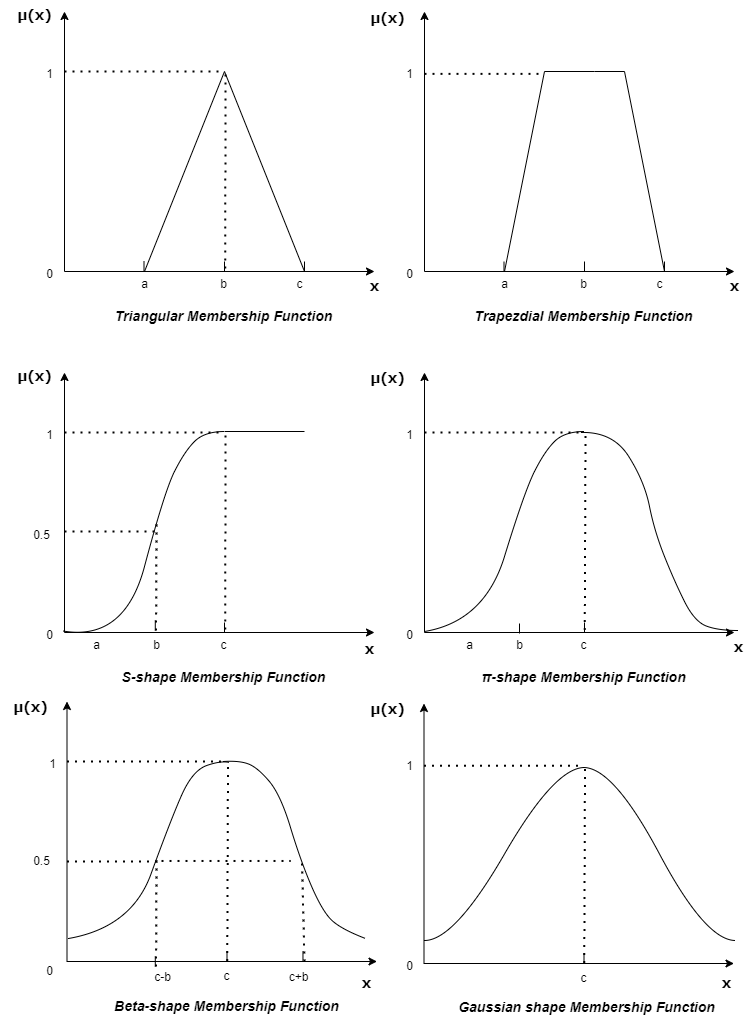
\includegraphics[width = 0.7 \textwidth]{img/membershipfunctions.png}
    \caption[Graphs of various types of fuzzy logic membership functions.]{Graphs of various types of fuzzy logic membership functions \cite{zain5}.}
    \label{fig:types_mf}
\end{figure}
Figure \ref{fig:types_mf} shows the shapes every membership function $\mu$ can take. Examples include suitable triangular or trapezoidal functions as well as Gaussian and bell-shaped functions. Considering the differential nature of gradient descent, it is recommended to utilise differentiable alternatives like Gaussian, sigmoidal, or generalised bell functions. The premise parameters, also known as antecedent parameters, are variables that shape these functions and undergo modifications during the back-propagation error correction process. Through findings from the literature review and the functions offered by MATLAB, the optimal membership functions for the features was chosen to be the Gaussian membership function. As a result, the Gaussian membership function was used to map all the inputs. It is important to note that these membership functions define the degree of membership of the input variables for only the specified range of inputs, i.e. anything outside the universe of $X$ will have a membership function of zero. Consequently, an ANFIS structure cannot extrapolate.  
\subsection{ANFIS Methods}
There are two different methods of designing an ANFIS: a Sugeno ANFIS and a Mamdani ANFIS. In the context of a drone control system, a Mamdani ANFIS could use several linguistic labels for each input variable (such as ``high'' or ``low'' altitude), with each label associated with a membership function. The output is also fuzzy in nature and defuzzification is needed to get a crisp output. This method is intuitively appealing and can be used to capture expert knowledge about how the drone should respond in different scenarios. However, it may be computationally intensive due to the requirement of defuzzification, which might limit its real-time applicability in high-speed scenarios, such as drone control. 

On the other hand, the Sugeno ANFIS method, instead of outputting a fuzzy set, produces a weighted average as its output. The Sugeno method typically requires less computational resources because the output is a polynomial function of the input variables, avoiding the need for defuzzification. In a drone control system, this could be advantageous when rapid responses to changing conditions are necessary, such as when the drone is manoeuvring in a complex environment. However, Sugeno systems can be more challenging to design and interpret because they don't use linguistic variables in the same way as Mamdani systems.

For the application of drone control, where computational efficiency and measurable, crisp outputs are used, the Sugeno design is likely to be the optimal ANFIS configuration. 

\subsection{ANFIS Types}
Type-1 and Type-2 ANFIS and they differ in how they handle uncertainty in the system.The difference between Type-1 and Type-2 fuzzy logic membership function is shown in Figure \ref{fig:type}.
The Type-1 ANFIS represents the more conventional and frequently used variant, employing standard fuzzy logic principles derived from Type-1 fuzzy sets. The degree of membership of an element in a fuzzy set is described by a membership function which can range between 0 and 1. This can be seen in Figure \ref{fig:type} with a single line indicating a crisp value relating $x_i$ (the range of possible values for a variable) and $\mu(x_i)$) representing the degree of membership for each value in the fuzzy set. In such a system, a variable's degree of membership to a fuzzy set is precise and ascertainable, making it effective for situations with explicit control rules. For instance, in the management of a drone control system, a Type-1 ANFIS, could contain distinct protocols dictating the drone's actions upon reaching specific altitudes or facing particular wind speeds. It delivers a single, definitive output for each respective input, assuming the same underlying conditions. Nevertheless, the Type-1 ANFIS may encounter difficulties when grappling with uncertainties or in the presence of noisy data or fluctuating environmental conditions - situations that are frequently encountered in real-world scenarios of drone navigation and control.

Type-2 FIS, on the other hand, have a fuzzy degree of membership i.e. can take values within a range. This is shown in Figure \ref{fig:type} where the shading values represent the uncertainty in the degree of membership for the different values of the variable. Type-2 FIS can be used for handling uncertain and vague input data, such as decision making in complex environments. This proves especially advantageous in intricate, volatile environments characterised by substantial uncertainty or noise, as it permits the system to assimilate and process this uncertainty instead of simply malfunctioning or generating an incorrect result.

For a drone control application, Type-2 ANFIS could be valuable in circumstances characterised by significant uncertainty or swift alterations in conditions, such as during a storm, or in regions with erratic wind flows. However, the literature review suggested that the level of uncertainty in the data set will be a key indicator of which ``type'' will be more effective. From the plots for the thrust and yaw in Figures \ref{fig:thrust_plot}\ref{fig:yaw_plot}, the optimal ANFIS configuration is likely to be a Type-1 design due to the minimal uncertainty. From the plots for the roll and pitch outputs in Figures \ref{fig:roll_plot} and \ref{fig:pitch_plot}, the uncertainty is higher and therefore a Type-2 design could be better in these cases. 
\begin{figure}[H]
    \centering
    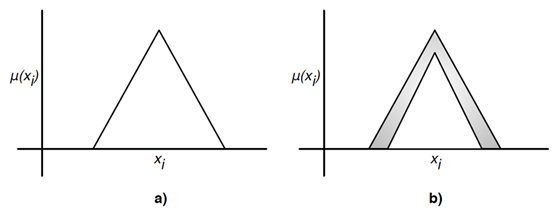
\includegraphics[width = 0.7 \textwidth]{img/Picture9.png}
    \caption[Graphs of fuzzy logic membership functions: a) Type-1; b) Type-2.]{Graphs of fuzzy logic membership functions: a) Type-1; b) Type-2 \cite{boxi8}.}
    \label{fig:type}
\end{figure}
\subsection{ANFIS Parameters Decision Making}
In order to determine the best design for the ANFIS for each output variable, we used the approach outlined in Figure \ref{fig:flow_fis}.
\begin{figure}[H]
    \centering
    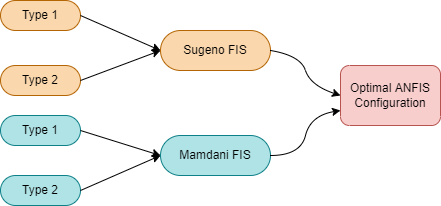
\includegraphics[width = 0.7\textwidth]{img/5.5drawio.png}
    \caption{Flowchart for ANFIS Configuration Decision making}
    \label{fig:flow_fis}
\end{figure}
The performance metric used to make these decisions was the Root Mean Square Error (RMSE) of the ANFIS. The RMSE is calculated in the following way:
\begin{equation}
\text{RMSE} = \sqrt{\frac{1}{n} \sum_{i=1}^{n} (y_i - \hat{y}_i)^2}
\end{equation}
Where $n$ is the total number of data points, $y_i$ is the actual value and $\hat{y}_i$ is the predicted value. The RMSE is a commonly used metric for measuring the differences between predicted and observed values. A lower RMSE value signifies a model with better predictive accuracy and there is a smaller difference between the actual values and the predicted values. 
\section{Implementation of Fuzzy Logic Controller}
A hybrid PID-ANFIS controller was implemented in Simulink. This approach checks each input at every time-step, to ensure that it is within the range of the FIS. If it is not, it will revert to the original PID controller. This is shown in Figure \ref{fig:Hybrid Control}. Although a hybrid PID-ANFIS controller was used, for clarity in results, this will be referred to as an ANFIS controller. This duality with PID control ensures the ANFIS controller is able to operate at every state, at the cost of program complexity and greater computational cost. The reason for this approach is because the fuzzy logic controller does not extrapolate due to the nature of the membership functions, as discussed in Section \ref{membership function}. If it receives an input that is outside of the original range of the training set, then the fuzzy logic controller is unable to provide an output. Although the Gaussian membership function is used, the membership function is actually limited by the range of the training data, contrary to what its name may suggest.
\begin{figure}[H]
    \centering
    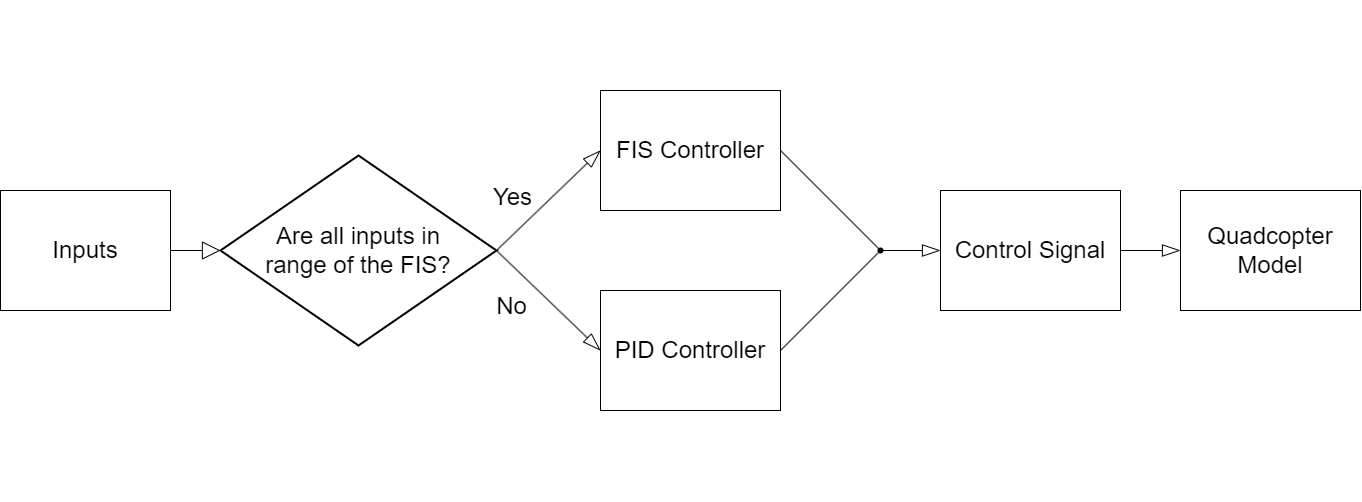
\includegraphics[width = \textwidth]{./img/hybrid_control.png}
    \caption{Flow chart for whether the FIS or PID controller will be used.}
    \label{fig:Hybrid Control}
\end{figure}
This was especially apparent when using the absolute position of the drone in the simulation environment, as it is nearly impossible to have a data-set encompassing all possible positions of the drone. To overcome this, the feature engineering of desired change in position, obtained by finding the difference between the desired position and current position, discussed in Section \ref{feature selection}, was used. As mentioned, this finds the relative position the drone wants to move to, while also reducing the number of inputs.

However, there were still edge cases where the inputs were not within the range of the fuzzy logic controller. This may be due to edge cases that were not covered in the training data, or new states that arise from the difference in behaviour of the fuzzy logic controller. This led to the implementation of the hybrid controller.

Another limitation is that MATLAB can only use neuro-adaptive learning methods to tune Type-1 Sugeno FIS with a single output as per MathWorks documentation. A workaround is that it is possible to tune the FIS, then convert it to another type, keeping the tuning. Tuning is an important step in FIS design, as it is used to optimise the membership functions. This is to obtain the membership functions which minimises the training error. This meant the options for controller design was very limited. Even though this was the case, various configurations were designed and tested even if some cannot be tuned. Two configurations for the fuzzy logic controller were made, one with four separate controllers, each with a single control signal output, with parameter selection and tuning; and one combined controller without parameter selection and tuning. These are shown in Figure \ref{fig:fis comparison}. This also provided insight on the improvement between a FIS with and without tuning. Through small simulation testing, the single controller configuration (Left of Figure \ref{fig:fis comparison}) was judged to be much less capable than the four seperate controller configuration, due to the inability to tune a single ANFIS for multiple outputs. 
\begin{figure}[H]
    \centering
    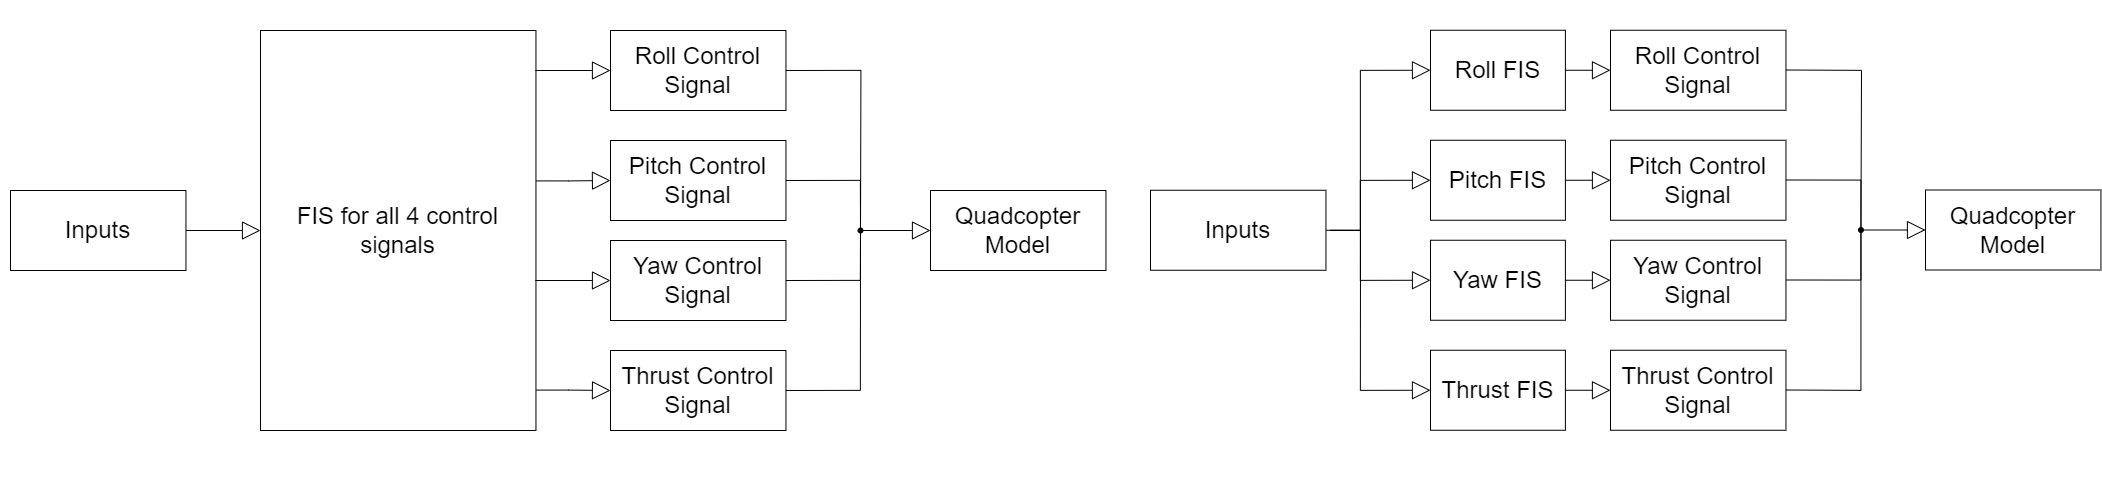
\includegraphics[width = \textwidth]{./img/fis_comparison.png}
    \caption{Left: Controller with single FIS and four outputs. Right: Four separate controllers with one output for each control signal.}
    \label{fig:fis comparison}
\end{figure}